\chapter{Background}

\section{Argumentation Frameworks}


Argumentation frameworks were first formally described by Dung in 1995 \cite{DUNG1995321}. They represent an information state, where various conclusions can be drawen from. An AF $G = (A, R)$ consists of two parameters: a set of arguments $A$, and a collection of relations $R$, called attacks which describe the conflicts between the arguments.

They are mostly used in the fields of \ac{AI}, f.e. in automated reasoning and logic programming \cite{AFINAIARLP, AFINAIARLPexample}. But do also find their applications in other fields like Natural Language Processing \cite{AFINNLP}, Trust and Reputation Systems \cite{AFINTaRS}, and even in Game Theory and Strategic Reasoning \cite{AFinGames}.

AFs are represented by directed graph, where the nodes are an abstraction of the arguments $A$, and the arrows represent the attacks $R$. Let us define an AF $G = (A, R)$ with the arguments 
\texttt{A=\{a, b, c, d, e\}} and the attacks 
\texttt{R=[(a,b),}
\texttt{(b,b),}
\texttt{(a,c),}
\texttt{(c,a),}
\texttt{(c,d),}
\texttt{(d,e),}
\texttt{(e,d)]}. With the arguments and attacks, we can create a directed graph \ref{af:backgroundAFexample1}
\begin{figure}[h]
    \centering
    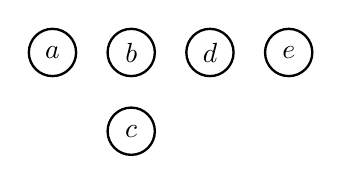
\begin{tikzpicture}
        % Singletons
        \def \ax{0}     \def \ay{0}
        \def \bx{1}     \def \by{0}
        \def \cx{1}     \def \cy{-1}
        \def \dx{2}     \def \dy{0}
        \def \ex{3}     \def \ey{0}

        \draw[line width=0.3mm] (\ax, \ay) circle (0.3) node[anchor=center]{$a$};
        \draw[line width=0.3mm] (\bx, \by) circle (0.3) node[anchor=center]{$b$};
        \draw[line width=0.3mm] (\cx, \cy) circle (0.3) node[anchor=center]{$c$};
        \draw[line width=0.3mm] (\dx, \dy) circle (0.3) node[anchor=center]{$d$};
        \draw[line width=0.3mm] (\ex, \ey) circle (0.3) node[anchor=center]{$e$};

        % Attacks
        \DrawAttackHorizontal{R}{\ax}{\ay}{\bx}{\by}
        \DrawSelfAttackRightSingleton{\bx}{\by}
        \DrawAttackDiagonal{NB}{\ax}{\ay}{\cx}{\cy}
        \DrawAttackDiagonal{PLR}{\cx}{\cy}{\dx}{\dy}
        \DrawAttackHorizontal{B}{\ex}{\ey}{\dx}{\dy}
    \end{tikzpicture}
    \caption{\ac{AF} G}
    \label{af:backgroundAFexample1}
\end{figure}

To be able to conclude something, out of an abstract AF, we need to define semantics. A semantic defines a subset of argument sets that satisfy the semantic-specific rules. Dung already defined different semantics \cite{Dung1995-DUNOTA-2} like \ac{cf}, \ac{adm} and \ac{stb}. According to Dungs definitions, a set \textit{S} is \ac{cf} if there are no attacks between the arguments in \textit{S}. The conflict-free set is mainly a building block for the other semantics, which means that the conflict-free set is always a superset of admissible and stable. In the example \ref{af:backgroundAFexample1} the $conflict-free$ sets are:
\texttt{\{a\}},
\texttt{\{c\}},
\texttt{\{d\}},
\texttt{\{e\}},
\texttt{\{a, d\}},
\texttt{\{a, e\}},
\texttt{\{c, e\}},


An admissible set is a conflict-free set, where each argument in \textit{S} has a defender in \textit{S}. In the example \ref{af:backgroundAFexample1} the $admissible$ sets are:
\texttt{\{a\}},
\texttt{\{c\}},
\texttt{\{e\}},
\texttt{\{a, d\}},
\texttt{\{a, e\}},
\texttt{\{c, e\}},

Finally, a stable set is a conflict-free set, if for every argument, which is not in \textit{S}, has an attacker which is in \textit{S}. In the example \ref{af:backgroundAFexample1} the $stable$ sets are:
\texttt{\{a, d\}},
\texttt{\{a, e\}},


The specific rules can be defined via a boolean formula. They can be used to encode the \acp{AF} to be solvable with different boolean solvers like \ac{ASP} \cite{DBLP:journals/corr/abs-1301-1388} or, as in our case, with a \ac{SAT-Solver} \cite{DBLP:journals/amai/AmgoudD13}. Unfortunately, drawing a conclusion from an AF can be challenging, e.g., it can be NP-complete and sometimes even be beyond NP to decide whether an argument is acceptable under a specific argumentation semantics \cite{DBLP:journals/ai/DvorakGRW23}.



\section{Clustering of Argumentation Frameworks}

\textit{TODO: What are clusters}

\textit{TODO: Why do we need clusters}

\textit{TODO: Definition of Semantics}

\textit{TODO: Complexity}


\section{SAT-Solver}

\textit{TODO: What are SAT-Solvers}

\textit{TODO: Complexity of SAT-Problems}

\textit{TODO: Where and how do we use SAT-Solvers in the research}

